\documentclass[11pt,a4paper]{article}

% === Packages (self-contained, no external input files) ===
\usepackage[utf8]{inputenc}
\usepackage[T1]{fontenc}
\usepackage{amsmath,amssymb,amsthm}
\usepackage{tikz}
\usepackage{pgfplots}
\pgfplotsset{compat=1.18}
\usepackage[margin=2.5cm]{geometry}
\usepackage{hyperref}
\hypersetup{colorlinks=true, linkcolor=blue!50!black, citecolor=blue!50!black, urlcolor=blue!50!black}

% === Custom macros (replace undefined registry macros) ===
\newcommand{\Hxi}{\mathcal{H}_{\xi}}
\newcommand{\Hlocal}{\mathcal{H}_{\mathrm{loc}}}
\newcommand{\Hdual}{\mathcal{H}_{\mathrm{dual}}}

% === Theorem-like environments ===
\theoremstyle{definition}
\newtheorem{definition}{Definition}[section]
\newtheorem{example}[definition]{Example}
\theoremstyle{remark}
\newtheorem{remark}[definition]{Remark}

\title{Companion 1: Die Kr\"ummungszerlegung\\
	\large Eine anschauliche Einf\"uhrung in die explizite Formel der Riemannschen Zeta-Funktion}
\author{Zahlenmodell Rigorous v2.0 -- Abitur-Companion}
\date{\today}

\begin{document}
	\maketitle
	\thispagestyle{empty}
	\tableofcontents
	\clearpage
	
	\section{Was ist die Kr\"ummungszerlegung?}\label{sec:krummung_einfuehrung}
	
	\begin{remark}[Zielgruppe und Scope]
		Dieses Companion-Dokument erkl\"art die Grundideen der Kr\"ummungszerlegung
		der expliziten Formel der Riemannschen Zeta-Funktion f\"ur Sch\"ulerinnen und
		Sch\"uler der Oberstufe. Wir verzichten auf komplizierte Beweise und
		konzentrieren uns auf Anschauung und Beispiele.
	\end{remark}
	
	\subsection{Die Grundidee: Kr\"ummung als Zugang zu Nullstellen}
	
	Stell dir vor, du m\"ochtest die Nullstellen einer komplexen Funktion finden,
	aber du kannst sie nicht direkt berechnen. Dann k\"onnte es hilfreich sein,
	indirekt vorzugehen: Betrachte die \textit{Kr\"ummung} des Graphen!
	
	\begin{definition}[Kr\"ummungsfeld (anschaulich)]
		Das \textit{Kr\"ummungsfeld} $\Hxi$ ist die zweite Ableitung des Logarithmus des
		Betrags der vervollst\"andigten Zeta-Funktion:
		\begin{equation}
			\Hxi(\sigma,t)\;:=\;\frac{d^2}{d\sigma^2}\log\lvert\xi(\sigma+it)\rvert^2
		\end{equation}
		Es beschreibt, wie stark sich die Funktion $\log\lvert\xi(s)\rvert^2$ an der Stelle
		$s = \sigma + it$ in Richtung der reellen Achse kr\"ummt.
	\end{definition}
	
	\begin{example}[Visualisierung des Kr\"ummungsfelds]
		Die Kr\"ummung einer Funktion gibt an, wie stark sie sich von einer Geraden unterscheidet.
		Bei einer Parabel $f(x) = x^2$ ist die Kr\"ummung \"uberall konstant, bei komplizierteren
		Funktionen \"andert sich die Kr\"ummung von Stelle zu Stelle.
	\end{example}
	
	\subsection{Warum ist das n\"utzlich?}
	
	Diese Betrachtung hat einen gro\ss en Vorteil: Wir k\"onnen Informationen \"uber die
	nicht-trivialen Nullstellen der Zeta-Funktion gewinnen!
	
	\begin{center}
		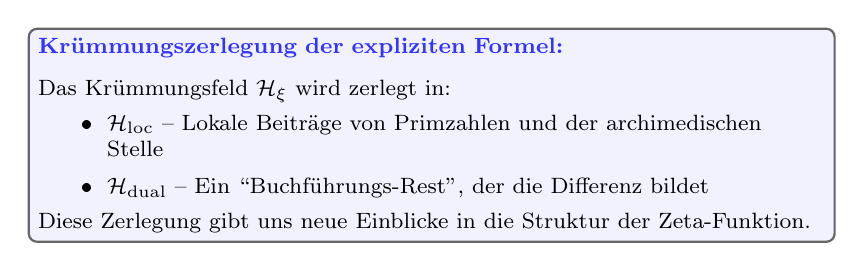
\begin{tikzpicture}
			\node[draw=black!60, thick, rectangle, rounded corners=3pt,
			fill=blue!5, text width=10cm, align=left,
			font=\footnotesize] at (0,0) {
				\textbf{\color{blue!80}Kr\"ummungszerlegung der expliziten Formel:}\\[0.2cm]
				Das Kr\"ummungsfeld $\Hxi$ wird zerlegt in:
				\begin{itemize}
					\item $\Hlocal$ -- Lokale Beitr\"age von Primzahlen und der archimedischen Stelle
					\item $\Hdual$ -- Ein ``Buchf\"uhrungs-Rest'', der die Differenz bildet
				\end{itemize}
				Diese Zerlegung gibt uns neue Einblicke in die Struktur der Zeta-Funktion.
			};
		\end{tikzpicture}
	\end{center}
	
	\section{Die explizite Formel verstehen}\label{sec:explizite_formel}
	
	\subsection{Was ist die explizite Formel?}
	
	Die explizite Formel ist eine der wichtigsten Entdeckungen in der analytischen Zahlentheorie.
	Sie verbindet zwei scheinbar unabh\"angige mathematische Welten:
	\begin{enumerate}
		\item Die Welt der Primzahlen (arithmetische Seite)
		\item Die Welt der Nullstellen der Zeta-Funktion (analytische Seite)
	\end{enumerate}
	
	\begin{remark}[Historischer Kontext]
		Die explizite Formel wurde von Riemann selbst entwickelt und sp\"ater von
		von Mangoldt pr\"azisiert. Sie bildet die Grundlage f\"ur den Beweis des Primzahlsatzes
		und spielt eine zentrale Rolle bei der Riemannschen Vermutung.
	\end{remark}
	
	\subsection{Die Formel in zwei Welten}
	
	Die explizite Formel kann als Gleichheit zweier Summen verstanden werden:
	
	\begin{center}
		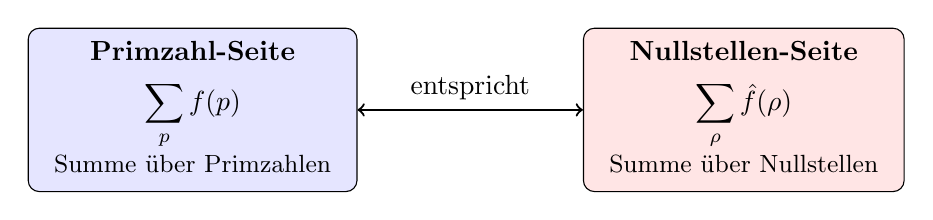
\begin{tikzpicture}
			\node[draw, fill=blue!10, rounded corners, minimum width=4cm, minimum height=2cm] (primside) at (-3.5,0) {
				\begin{tabular}{c}
					\textbf{Primzahl-Seite} \\[4pt]
					$\displaystyle\sum_{p} f(p)$ \\[4pt]
					\small Summe \"uber Primzahlen
				\end{tabular}
			};
			\node[draw, fill=red!10, rounded corners, minimum width=4cm, minimum height=2cm] (zeroside) at (3.5,0) {
				\begin{tabular}{c}
					\textbf{Nullstellen-Seite} \\[4pt]
					$\displaystyle\sum_{\rho} \hat{f}(\rho)$ \\[4pt]
					\small Summe \"uber Nullstellen
				\end{tabular}
			};
			\draw[<->, thick] (primside) -- (zeroside) node[midway, above] {entspricht};
		\end{tikzpicture}
	\end{center}
	
	In Tehranis Paper wird eine spezielle Version dieser Formel betrachtet, die sich auf
	die zweite Ableitung des Logarithmus der $\xi$-Funktion konzentriert.
	
	\section{Die Kr\"ummungszerlegung}\label{sec:kruemmungszerlegung}
	
	\subsection{Zwei Komponenten der Kr\"ummung}
	
	Das Kr\"ummungsfeld $\Hxi$ wird in zwei Teile zerlegt:
	
	\begin{definition}[Lokale Kr\"ummung]
		$\Hlocal$ repr\"asentiert die Beitr\"age von:
		\begin{itemize}
			\item Archimedischer Stelle: $\psi_1(\sigma) = \frac{1}{8}\psi^{(1)}\!\bigl(\frac{\sigma}{2}\bigr)$
			\item Endlichen Stellen (Primzahlen): $\sum_{p \leq \kappa} V_p(\sigma)$
		\end{itemize}
		
		Dabei ist $V_p(\sigma) = 4(\log p)^2 \dfrac{p^{-2\sigma}}{(1-p^{-2\sigma})^2}$ der Beitrag jeder Primzahl~$p$.
	\end{definition}
	
	\begin{definition}[Buchf\"uhrungs-Rest]
		$\Hdual$ ist die Differenz zwischen dem Gesamtfeld und der lokalen Kr\"ummung:
		\begin{equation}
			\Hdual(\sigma,t,\kappa) = \Hxi(\sigma,t) - \Hlocal(\sigma,\kappa)
		\end{equation}
	\end{definition}
	
	\subsection{Visualisierung der Komponenten}
	
	\begin{center}
		\begin{tikzpicture}[scale=0.85]
			% Gesamtfeld
			\begin{scope}[shift={(-5.5,3)}]
				\draw[->] (-2.5,0) -- (2.5,0) node[right] {\small $\sigma$};
				\draw[->] (0,-0.5) -- (0,3) node[above] {\small $\Hxi$};
				\draw[thick, blue, domain=-2:2, samples=80] plot (\x, {(\x)^2/3 + 1/((\x)^2+0.3)});
				\node[blue, font=\small] at (2,2.5) {$\Hxi(\sigma,t)$};
			\end{scope}
			
			% Lokale Komponente
			\begin{scope}[shift={(5.5,3)}]
				\draw[->] (-2.5,0) -- (2.5,0) node[right] {\small $\sigma$};
				\draw[->] (0,-0.5) -- (0,3) node[above] {\small $\Hlocal$};
				\draw[thick, red, domain=-2:2, samples=80] plot (\x, {(\x)^2/3 + 0.5});
				\node[red, font=\small] at (2,2.5) {$\Hlocal(\sigma,\kappa)$};
			\end{scope}
			
			% Rest-Komponente
			\begin{scope}[shift={(0,-2.5)}]
				\draw[->] (-2.5,0) -- (2.5,0) node[right] {\small $\sigma$};
				\draw[->] (0,-1) -- (0,3) node[above] {\small $\Hdual$};
				\draw[thick, green!60!black, domain=-2:2, samples=80] plot (\x, {1/((\x)^2+0.3) - 0.5});
				\node[green!60!black, font=\small] at (2.5,1.5) {$\Hdual(\sigma,t,\kappa)$};
			\end{scope}
			
			% Zusammenhang-Pfeile
			\node at (0,4.2) {\small $\Hxi = \Hlocal + \Hdual$};
			\draw[->, thick, purple, dashed] (-2.5,1.5) -- (-1.5,-0.5);
			\draw[->, thick, purple, dashed] (2.5,1.5) -- (1.5,-0.5);
		\end{tikzpicture}
	\end{center}
	
	\section{Die Hauptergebnisse des Papers}\label{sec:hauptergebnisse}
	
	\subsection{Vier zentrale Beweise}
	
	Tehrani beweist vier wichtige Eigenschaften:
	
	\begin{enumerate}
		\item \textbf{Lokale Positivit\"at}: $V_p(\sigma) \geq 0$ f\"ur alle Primzahlen $p$ und alle $\sigma > 0$.
		\item \textbf{Nicht-Negativit\"at der lokalen Kr\"ummung}: $\Hlocal(\sigma,\kappa) \geq 0$ f\"ur alle $\sigma > 0$.
		\item \textbf{Divergenz auf der kritischen Linie}: Auf $\sigma = \frac{1}{2}$ w\"achst $\Hlocal$ mit der
		Ordnung $(\log\kappa)^2$ ins Unendliche.
		\item \textbf{Konvergenz \"uber der kritischen Linie}: F\"ur $\sigma > \frac{1}{2}$ konvergiert
		$\Hlocal(\sigma,\kappa)$ gegen einen endlichen Wert, wenn $\kappa \to \infty$.
	\end{enumerate}
	
	\begin{remark}[Phasen\"ubergang]
		Die kritische Linie $\sigma = \frac{1}{2}$ bildet also eine Art Phasengrenze zwischen
		Divergenz und Konvergenz der lokalen Kr\"ummungssumme!
	\end{remark}
	
	\subsection{Numerische Beobachtungen}
	
	Neben den Beweisen macht Tehrani auch numerische Beobachtungen:
	
	\begin{enumerate}
		\item \textbf{Kompensation abseits der kritischen Linie}: Bei $\sigma = 0.3$ und $\kappa = 1300$
		ist $\Hlocal \approx 915$, w\"ahrend $\Hxi \approx 0.09$. Das bedeutet, dass $\Hdual$ die
		lokale Kr\"ummung zu mehr als 99{,}99\% ausgleicht!
		\item \textbf{Singul\"are Spitzen nahe der Nullstellen}: Auf der kritischen Linie zeigt $\Hxi$
		scharfe Spitzen nahe den nicht-trivialen Nullstellen. Zum Beispiel:
		\begin{itemize}
			\item $\Hxi\bigl(\tfrac{1}{2}, 14.13\bigr) \approx +89\,577.92$ (nahe der ersten Nullstelle)
			\item $\Hxi\bigl(\tfrac{1}{2}, 21.02\bigr) \approx +480\,754.91$ (nahe der zweiten Nullstelle)
		\end{itemize}
	\end{enumerate}
	
	\begin{center}
		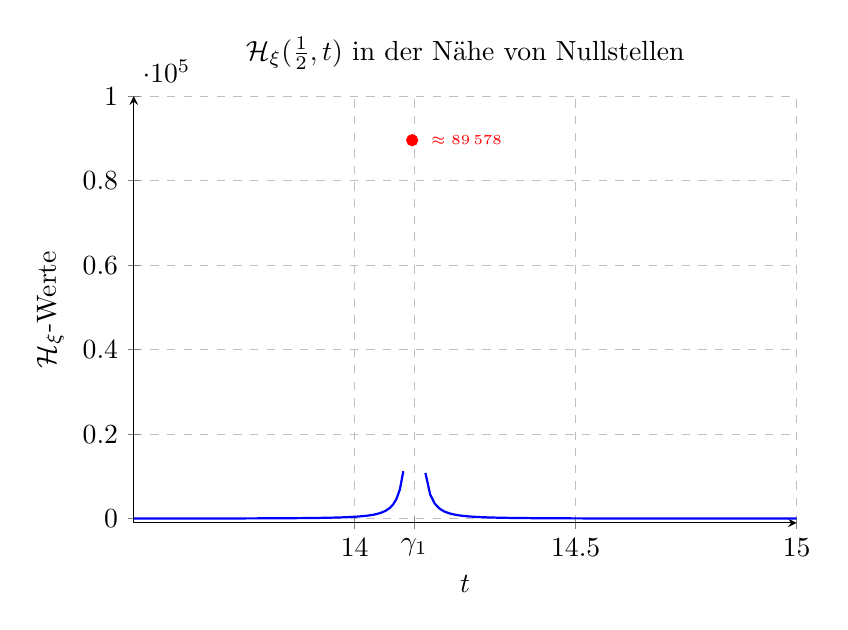
\begin{tikzpicture}
			\begin{axis}[
				title={$\Hxi(\frac{1}{2}, t)$ in der N\"ahe von Nullstellen},
				xlabel={$t$},
				ylabel={$\Hxi$-Werte},
				xmin=13.5, xmax=15,
				ymin=-1000, ymax=100000,
				xtick={14, 14.1347, 14.5, 15},
				xticklabels={14, $\gamma_1$, 14.5, 15},
				axis lines=left,
				ymajorgrids=true,
				xmajorgrids=true,
				grid style=dashed,
				width=10cm,
				height=7cm,
				]
				
				\addplot[
				color=blue,
				mark=none,
				domain=13.5:14.11,
				samples=80,
				thick,
				] {80000/((x-14.1347)^2*10000 + 1)};
				
				\addplot[
				color=blue,
				mark=none,
				domain=14.16:15,
				samples=80,
				thick,
				] {80000/((x-14.1347)^2*10000 + 1)};
				
				\addplot[mark=*, mark size=2pt, color=red] coordinates {(14.13, 89577.92)};
				\node[right, font=\tiny, red] at (axis cs:14.15, 89577) {$\approx 89\,578$};
				
			\end{axis}
		\end{tikzpicture}
	\end{center}
	
	\section{Die Bedeutung f\"ur die Riemannsche Vermutung}\label{sec:bedeutung}
	
	\subsection{Was ist die Riemannsche Vermutung?}
	
	Die Riemannsche Vermutung ist eines der wichtigsten ungel\"osten Probleme der Mathematik.
	Sie besagt:
	
	\begin{remark}[Die Riemannsche Vermutung]
		Alle nicht-trivialen Nullstellen der Zeta-Funktion liegen auf der kritischen Linie
		$\sigma = \frac{1}{2}$.
	\end{remark}
	
	Seit \"uber 160 Jahren versuchen Mathematiker, diese Vermutung zu beweisen. Ihre
	Richtigkeit h\"atte tiefgreifende Konsequenzen f\"ur unser Verst\"andnis der Primzahlverteilung.
	
	\subsection{Wie h\"angt die Kr\"ummungszerlegung damit zusammen?}
	
	Tehranis Ansatz bietet einen neuen Blickwinkel:
	
	\begin{enumerate}
		\item Die lokale Kr\"ummung $\Hlocal$ ist \"uberall positiv.
		\item Auf der kritischen Linie divergiert $\Hlocal$.
		\item Abseits der kritischen Linie heben sich $\Hlocal$ und $\Hdual$ fast vollst\"andig auf.
		\item Auf der kritischen Linie zeigt $\Hxi$ scharfe Spitzen nahe den Nullstellen.
	\end{enumerate}
	
\end{document}